\documentclass{article}

\title{On The Stern-Gerlach Experiment}
\author{Danial Yahyazadeh\footnote{danial.yahyazadeh@gmail.com}\\ 
\small{
ISK Foundation}%
\footnote{\href{https://iskportal.com/}{ISK Portal}}
}
\date{September 2024}

\begin{document}


\maketitle

\begin{abstract}
    We are here to create content for \textbf{Independent Society of Knowledge}, So start with the Stern-Gerlach experiment!
\end{abstract}

\section{Introduction}
One of the best experiments on explaining quantum behavior is the Stern-Gerlach experiment, which concerns the spin of a particle like an electron. It helps us understand that spin is quantized \& the concept of collapsing wave function.

\section{The Experiment Apparatus \& Its Setup}
Stern-Gerlach apparatus was first time invented  by O. Stern in 1921  \& later in collaboration with W. Gerlach in 1922; includes one oven of silver atoms with a hole on it that atoms can escape through (1) \& out of the oven there exists some beam splitter to make a straight beam of silver atoms as (2) in figure
\ref{Stern-Gerlach Experiment}.

Then this beam is directed to an inhomogeneous magnetic field that two magnets with different shapes can produce, as shown in (3) \ref{Stern-Gerlach Experiment}.

At last, we can see a screen after the magnets the results of the experiment be shown on it (5).
\begin{figure}[h]
    \centering
    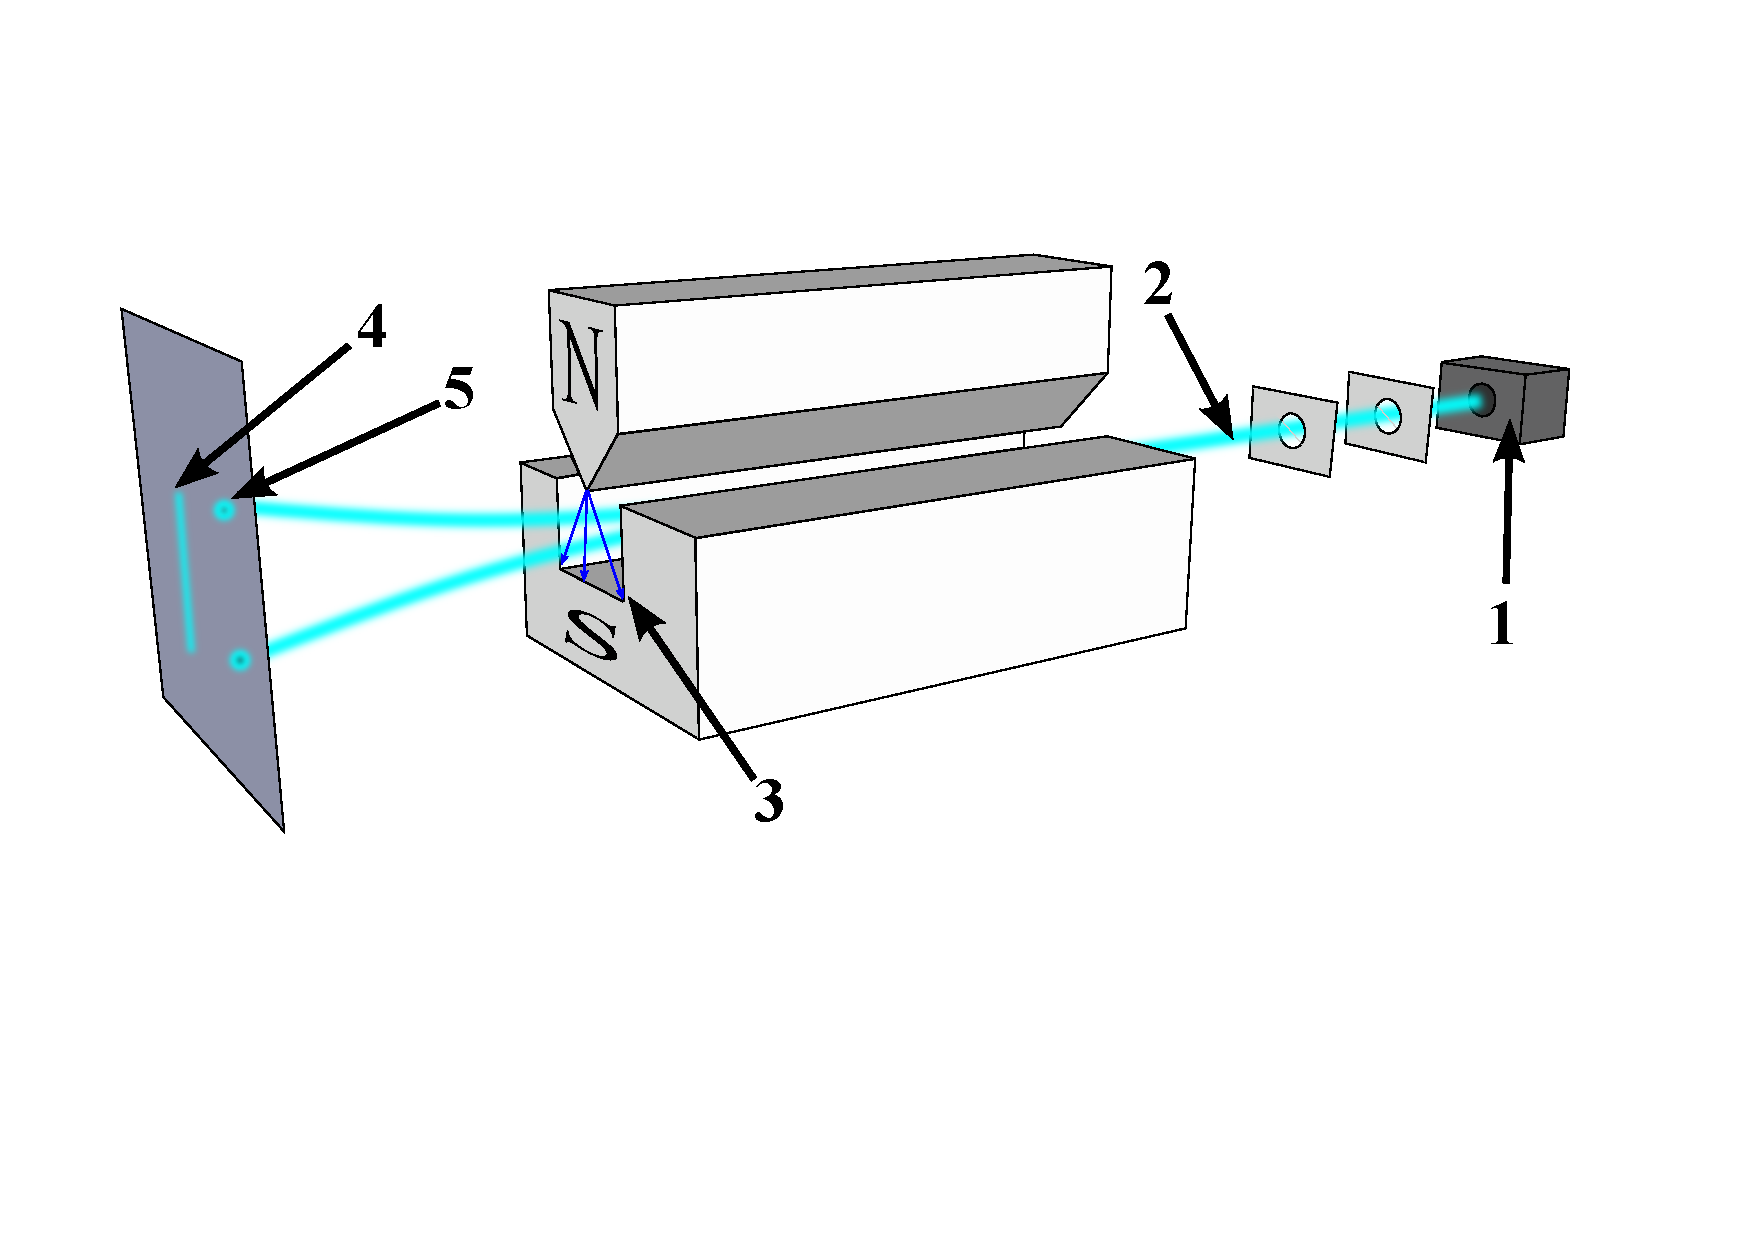
\includegraphics[width=0.5\linewidth]{Stern-Gerlach_experiment_svg.pdf}
    \caption{Stern-Gerlach Experiment}
    \label{Stern-Gerlach Experiment}
\end{figure}

\section{What Stern-Gerlach Experiment Can Tell Us}

\subsection{Spin Is Quantized!}
 The silver atoms (Ag) are employed because of their uncoupled electron (47th) in the last atomic layer $(s5)$ where its intrinsic magnetic moment is $\vec{\mu}$, so that:
 \begin{equation}
     \vec{\mu}\propto \vec{S}.
 \end{equation}
 Then according to Hamiltonian of interaction between the intrinsic magnetic moment of electron \& magnetic field  ($H=-\vec{\mu}\cdot\vec{B}$), if the $B$ is directed to $z$ axis, this electron experiences a force like as:
 \begin{equation}
     F_{z}=\frac{\partial}{\partial z}\left(\vec{\mu}\cdot\vec{B}\right)\simeq\mu_{z}\frac{\partial B_z}{\partial z}.
 \end{equation}
According to classical physics, the magnetic moment of an electron must be $-a<\mu_z<a$ or continuous value, then under the above force we can see that the (4) pattern in the figure \ref{Stern-Gerlach Experiment} must be shown to us. But the real result is different; the (5) pattern in figure \ref{Stern-Gerlach Experiment} appears! So we can deduce from this result that the magnetic moment or \textbf{intrinsic spin} of the electron must be a discrete value which is $S_z=\pm\frac{\hbar}{2}$ \cite{Sakurai_Napolitano_2020}.

Then the most important result of the Stern-Gerlach experiment is that the electron has spin \& its value is discrete or better to say that \textbf{Spin Is Quantized!}

\subsection{Sequential Stern-Gerlach Experiments \small{(Collapsing of Wave Function)}}
\begin{figure}[t]
    \centering
    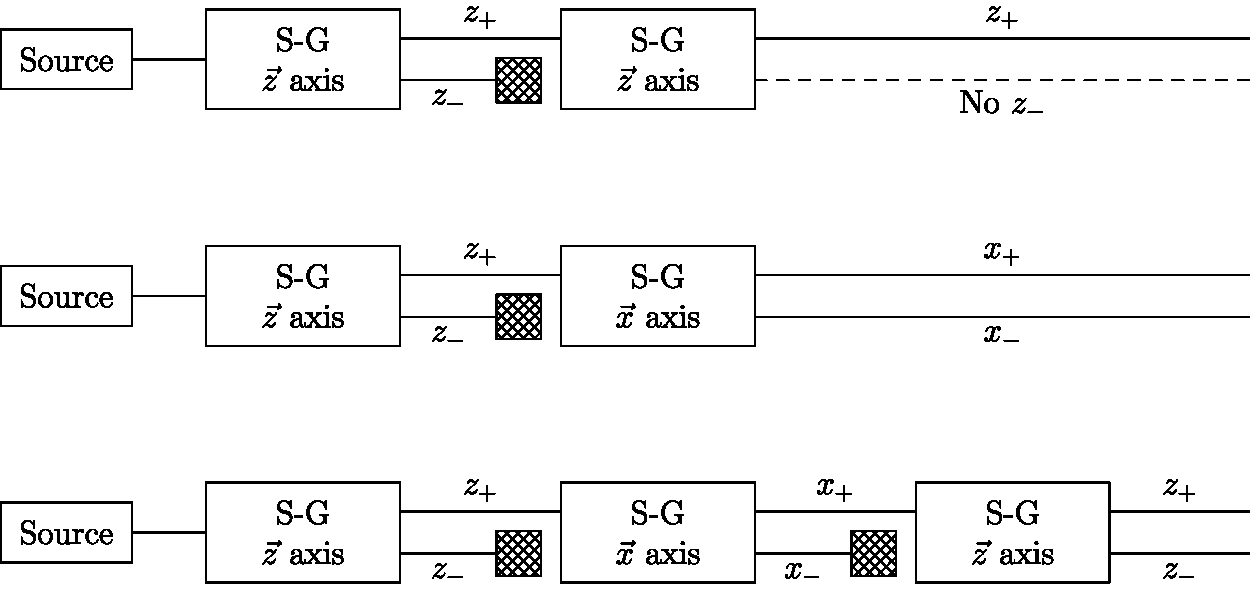
\includegraphics[width=0.7\linewidth]{Sg-seq.pdf}
    \caption{Sequential Stern-Gerlach Experiments}
    \label{Sequential Stern-Gerlach Experiments}
\end{figure}
The strangest thing about the quantum nature is when it occurs that we do sequential Stern-Gerlach Experiments as we can see in figure \ref{Sequential Stern-Gerlach Experiments}. We can itemize it in 3 ways \cite{bookjeanbricmont}:
\begin{enumerate}
    \item A beam with state $\ket{\psi_0}$ enter to a $z$ axis apparatus next two beam exit from it with probabilities:
    \begin{align}
P\left(S^{\pm}_{z}\right)=|\braket{\psi_0|S^{\pm}_{z}}|^2=\frac{1}{2},
    \end{align}
    then if we do it again by a second $z$ axis apparatus and just enter the $S^{+}_{z}$, we can see that the only $S^{+}_{z}$ component beam exit from the second apparatus with probability:
    \begin{equation}
        P\left(S^{+}_{z}\right)=|\braket{\psi_0|S^{+}_{z}}|^2|\braket{S^{+}_{z}|S^{+}_{z}}|^2=\frac{1}{2},
    \end{equation}
    As we expected classically.
    \item As before first a $z$ axis apparatus and after that there is a   $x$ axis apparatus on the way of $S^{+}_{z}$ component beam, the final result is two beams of $S^{\pm}_{x}$ components with probability:
    \begin{equation}
P\left(S^{\pm}_{x}\right)=|\braket{\psi_0|S^{+}_{z}}|^2|\braket{S^{+}_{z}|S^{\pm}_{x}}|^2=\frac{1}{4},
    \end{equation}
    as we expected.
    \item Finally do the same as item no.2 just after the $x$ axis apparatus put a $z$ axis apparatus again on the way of $S^{x}_{z}$ beam, before going further we can deduce logically that like as item no.1 the only beam exited from the $z$ axis apparatus is $S^{+}_{z}$, but in the real world our classical logic is not correct; The real \& strangest result for us occurs in such a way that we have two beams with $S^{\pm}_z$ components with probability as below:
    \begin{equation}
P\left(S^{\pm}_{z}\right)=|\braket{\psi_0|S^{+}_{z}}|^2|\braket{S^{+}_{z}|S^{+}_{x}}|^2|\braket{S^{+}_{x}|S^{\pm}_{z}}|=\frac{1}{8}.
    \end{equation}
    This is what we call it \textbf{collapsing of wave function} or better say any observation on quantum systems perturbed the results \& the different apparatus collapses the first wave function then if we do experiment with the first apparatus make a new wave function, which is unknown to us in classical physics because it's a quantum behavior!
\end{enumerate}

\section{Conclusion}
We can see in this brief text that the Stern-Gerlach experiment shows us the Spin of a quantum particle is quantized \& the sequential Stern-Gerlach experiment changes our classical thoughts with its amazing results.

\bibliographystyle{plain}  
\bibliography{bibfile.bib}  
\end{document}
